\documentclass[addpoints]{exam}

\makeatletter % Lagfæring fyrir nýjar útgáfur af TeXLive
\expandafter\providecommand\expandafter*\csname ver@framed.sty\endcsname
{2003/07/21 v0.8a Simulated by exam}
\makeatother

\usepackage[top=2cm, bottom=2cm, left=1cm, right=1cm]{geometry}
\usepackage[utf8]{inputenc}
\usepackage[icelandic]{babel}
\usepackage[T1]{fontenc}
% \usepackage[sc]{mathpazo}
\usepackage{helvet} \renewcommand\familydefault{\sfdefault}

\usepackage[parfill]{parskip}
\usepackage{tabularx}
\usepackage{multirow}
\usepackage{multicol}
\usepackage{graphicx}
\usepackage{enumerate}
\usepackage{amsmath, amsfonts, amssymb, amsthm}
\usepackage{minted} %Minted and configuration
\usepackage{afterpage}
\usepackage{scrextend}

\usepackage[pdftex,bookmarks=true,colorlinks=true,pdfauthor={Eirikur Ernir Thorsteinsson},linkcolor=blue,urlcolor=blue]{hyperref}

\setcounter{secnumdepth}{-1} 
\hyphenpenalty=5000

\newcommand\blankpage{%
    \null
    \thispagestyle{empty}%
    \addtocounter{page}{-1}%
    }

\usemintedstyle{default}
\renewcommand{\theFancyVerbLine}{\sffamily \arabic{FancyVerbLine}}
\author{}
\date{}

\footer{}{}{}

\setcounter{secnumdepth}{-1} 

\qformat{\large \textbf Spurning \thequestion \phantom{M}(\totalpoints \phantom{l}stig) \hfill}
\renewcommand{\solutiontitle}{\noindent\textbf{Svar:}\par\noindent}
\renewcommand{\points}{stig}
\renewcommand{\questionshook}{\setlength{\itemsep}{0.5cm}}
\hqword{Spurning:}
\hpword{Stig í boði:}
\hsword{Stig:}
\htword{Samtals}

\title{TÖL104G Stærðfræðimynstur í tölvunarfræði - lokapróf}
\author{}
\date{8. desember 2017}

\pagestyle{headandfoot}
\firstpageheader{TÖL104G}{Lokapróf//Final exam}{8. desember 2017}
\firstpagefooter{}{Bls. \thepage\ af \numpages}{}
\runningfooter{}{Bls. \thepage\ af \numpages}{}
\setlength{\columnsep}{0.5cm}

\changefontsizes{14pt}

% \printanswers
\begin{document}

% \thispagestyle{empty}
Fullt nafn//Full name: \vspace*{1mm} \hrule

\begin{center}
    \begin{minipage}{\textwidth}
    
    \vspace{0.7cm}
    \paragraph{Leiðbeiningar} Á þessu prófi eru \numquestions\ spurningar sem samtals gefa \numpoints\ stig. Leyfileg hjálpargögn eru reiknivél og ein A4 blaðsíða af glósum.
    
    Heftið verður skannað inn í tölvu til yfirferðar. Vinsamlegast forðist ljósa blýanta, ekki rífa eða krumpa heftið og ekki bæta við blaðsíðum. 
    
    Til að svara krossaspurningum skal nota svartöfluna hér að neðan. Merkið vandlega við einn möguleika fyrir hverja spurningu. Ekki er dregið frá fyrir röng svör. 
    
    Til að svara almennum spurningum skal skrifa inn í svæðið sem fylgir strax á eftir hverri spurningu. Þurfi að koma viðbótarupplýsingum til skila skal skrifa það í rammana á öftustu blaðsíðunum. Aðrir hlutar heftisins, sér í lagi bakhliðar, \emph{verða ekki lesnir}.
    
    Dæmin á þessu prófi eru misþung. Þau eru ekki sett fram í erfiðleikaröð.
    
    \vspace{0.7cm}
    

    \begin{multicols}{2}

        \paragraph{Instructions} This exam consists of \numquestions\ questions worth a total of \numpoints\ points. You may bring a calculator and one A4 sheet of notes to the exam.
        
        This exam will be digitally scanned for grading. Please avoid light pencils, tearing or crumpling the pages and adding pages. 
        
        To answer multiple choice questions, use the answer table to the right. Carefully mark one option for each question. Points are not deducted for wrong choices. 
        
        To answer general questions, write within the area immediately following each question. If additional space is needed, write within the frames on the last two pages. Other parts of the exam sheets, particularly the overleaf, \emph{will not be read}.
        
        Some questions on this exam are less difficult than others, they are not ordered by difficulty.

        \begin{center}
            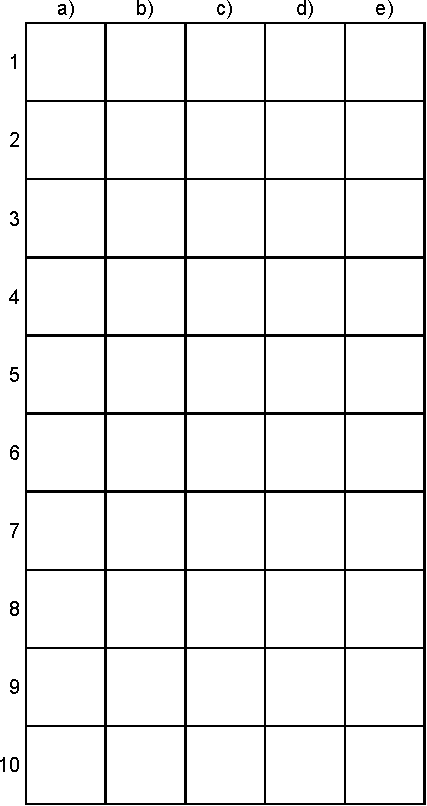
\includegraphics[width=0.7\linewidth]{Pics/svartafla}
        \end{center}
    \end{multicols}    
    \end{minipage}

\end{center}

\begin{questions}
        
\section{Krossaspurningar//Multiple Choice Questions}

\question[3] 

\textbf{(Ísl)} Yrðingarnar $p \to q$ og $\lnot q \to \lnot p$ eru jafngildar. Sönnun sem notar þetta jafngildi kallast\ldots

\textbf{(En)} The propositions $p \to q$ and $\lnot q \to \lnot p$ are equivalent. A proof that makes use of this equivalence is referred to as\ldots

\begin{enumerate}[a)]
    \item Bein sönnun // a direct proof
    \item Sönnun með mótskilyrðingu // a proof by contraposition % Rétt
    \item Sönnun með mótsögn // a proof by contradiction
    \item Sönnun með mótdæmi // a proof by counterexample
    \item Afsönnun // a debunking
\end{enumerate}

\question[3]
\textbf{(Ísl)} Látum $C(x)$ vera staðhæfinguna ``$x$ á kött'', $D(x)$ vera staðhæfinguna ``$x$ á hund'' og $F(x)$ vera staðhæfinguna ``$x$ á mörð''. Látum óðalið vera mengi nemenda í þessu námskeiði. Setjið staðhæfinguna ``Einhver nemandi í þessu námskeiði á kött og mörð en ekki hund'' fram með því að nota $C(x), D(x), F(X)$, rökvirkja og magnara.
    
\textbf{(En)} Let $C(x)$ be the statement ``x has a cat,'' let $D(x)$ be the statement ``x has a dog,'' and let $F(x)$ be the statement ``x has a ferret,''. Let the domain consist of all students in this class. Express the statement ``Some student in your class has a cat and a ferret, but not a dog.'' in terms of $C(x), D(x), F(x)$, quantifiers, and logical connectives.

\begin{enumerate}[a)]
    \item $\exists x(C(x) \lor F(x) \lor \lnot D(x))$
    \item $\exists x(C(x) \land F(x) \land \lnot D(x))$ % Rétt
    \item $\exists x(C(x) \land F(x) \land D(x))$
    \item $\lnot \exists x(C(x) \land F(x) \land D(x))$
    \item $\forall x(C(x) \lor F(x) \lor \lnot D(x))$
\end{enumerate}

\newpage

\question[3] 

\textbf{(Ísl)} Hversu mörg stök inniheldur veldismengi mengis með $n$ stökum?

\textbf{(En)} How many elements does the power set of a set with $n$ elements have?

\begin{enumerate}[a)]    
    \item $1$
    \item $n$
    \item $n^2$
    \item $2^n$ % Rétt
    \item $n^n$
\end{enumerate}

\question[3] 

\textbf{(Ísl)} Hvert er minnsta samfeldi $2\cdot 3 \cdot 5^2 \cdot 11$ og $2^3 \cdot 7 \cdot 11 \cdot 13$?

\textbf{(En)} What is the least common multiple of $2\cdot 3 \cdot 5^2 \cdot 11$ and $2^3 \cdot 7 \cdot 11 \cdot 13$?

\begin{enumerate}[a)]
    \item $2^3\cdot 3 \cdot 5^2 \cdot 7 \cdot 11 \cdot 13$ % Rétt
    \item $2\cdot 11$
    \item $2\cdot 3 \cdot 5 \cdot 7 \cdot 11 \cdot 13$
    \item $2^4\cdot 3 \cdot 5^2 \cdot 7 \cdot 11^2 \cdot 13$
    \item $42$
\end{enumerate}

\question[3]

\textbf{(Ísl)} Endurkvæmt fall er gefið, ásamt upphafsskilyrðum. Hvað er $f(3)$?

\[
    f(n+1) = 2f(n) + 3, f(0) = 3
\]

\textbf{(En)} A recursive function is given above, along with initial conditions. What is the value of $f(3)$?

\begin{enumerate}[a)]
    \item 4
    \item 9
    \item 21
    \item 45
    \item 93
\end{enumerate}

\newpage

\question[3] 

\textbf{(Ísl)} Gefin eru vensl á mengi heiltalnanna.

\[
    R = \{(a,b)|a=b+1\}
\]

Hvert af eftirfarandi er rétt lýsing á eiginleikum þeirra?

\textbf{(En)} Consider the relation on the set of integers described above. Which of the following is a correct desription of its properties?

\begin{enumerate}[a)]
    \item Sjálfhverf, ekki samhverf, ekki andsamhverf, ekki gegnvirk // Reflexive, not symmetric, not antisymmetric, not transitive    
    \item Ekki sjálfhverf, samhverf, ekki andsamhverf, ekki gegnvirk // Not reflexive, symmetric, not antisymmetric, not transitive
    \item Ekki sjálfhverf, ekki samhverf, andsamhverf, ekki gegnvirk // Not reflexive, not symmetric, antisymmetric, not transitive % Rétt
    \item Ekki sjálfhverf, ekki samhverf, ekki andsamhverf, gegnvirk // Not reflexive, not symmetric, not antisymmetric, transitive
    \item Ekki sjálfhverf, ekki samhverf, ekki andsamhverf, ekki gegnvirk // Not reflexive, not symmetric, not antisymmetric, not transitive
\end{enumerate}

\question[3] 

\textbf{(Ísl)} Hver er litunartala hjólsins $W_n$?

\textbf{(En)} What is the chromatic number of the wheel $W_n$?

\begin{enumerate}[a)]
    \item 3
    \item 4
    \item 3 sé $n$ slétt tala, 4 sé $n$ oddatala//3 if $n$ is even, 4 if $n$ is odd % Rétt
    \item 4 sé $n$ slétt tala, 3 sé $n$ oddatala//4 if $n$ is even, 3 if $n$ is odd
    \item 2
\end{enumerate}

\newpage

\question[3]

\textbf{(Ísl)} Hver er summa stiga allra hnúta í $n$ hnúta tré?

\textbf{(En)} What is the sum of the degrees of the vertices of a tree with $n$ vertices?

\begin{enumerate}[a)]
    \item $n-1$
    \item $n$
    \item $2n$
    \item $n-2$
    \item $2n-2$ % Rétt
\end{enumerate}

\question[3]

\textbf{(Ísl)} Hvert eftirfarandi reiknirita finnur léttasta spanntré í neti?

\textbf{(En)} Which of the following algorithms finds a graph's minimum spanning tree?

\begin{enumerate}[a)]
    \item Reiknirit Prims // Prim's algorithm % Rétt
    \item Reiknirit Dijkstras // Dijkstra's algorithm
    \item Reiknirit Evklíðs // Euclid's algorithm
    \item Dýptarleit // Depth-first search
    \item Breiddarleit // Breadth-first search
\end{enumerate}

\question[3]

\textbf{(Ísl)} Mengi þeirra ákvörðunarvandamála sem leysanleg eru á margliðutíma er venjulega kallað

\textbf{(En)} The set of decision problems that can be solved in polynomial time is usually called

\begin{enumerate}[a)]
    \item $P$ % Rétt
    \item $NP$
    \item $NP$-complete
    \item $NP$-hard
    \item $L$
\end{enumerate}

\newpage

\section{Almennar spurningar//General Questions}

\question[10] 

\textbf{(Ísl)} Sýnið að $(p \to r) \lor (q \to r)$ og $(p \land q) \to r$ séu jafngildar á tvenna vegu.

\textbf{(En)} Show that $(p \to r) \lor (q \to r)$ and $(p \land q) \to r$ are logically equivalent in two ways.

a) Sýnið með því að nota sanntöflu // Show it using a truth table

\makeemptybox{\stretch{1}}

\newpage

b) Sýnið með því að nota þekkt jafngildi. Ekki þarf að nefna nöfn jafngildanna, en sýnið aðferð svo skýrt sé. // Show it using known logical equivalences. The names of the used equivalences do not need to be mentioned, but show the steps involved in your work.

\makeemptybox{\stretch{1}}

\newpage
\question[10]

\textbf{(Ísl)} Sýnið að// \textbf{(En)} Show that
a) $x^2 + 4x + 3$ sé $O(x^2)$//$x^2 + 4x + 3$ is $O(x^2)$

\makeemptybox{\stretch{1}}

\newpage

b) $x^3$ sé ekki $O(x^2 + 4x + 3)$//$x^3$ is not $O(x^2 + 4x + 3)$

\makeemptybox{\stretch{1}}

\newpage

\question[10] 

\textbf{(Ísl)} Notið þrepun til að sanna að \[1\cdot 2 + 2 \cdot 3 + \ldots + n(n+1) = \frac{n(n+1)(n+2)}{3}\] fyrir allar jákvæðar heiltölur $n$. Taktu fram hver þrepunarforsendan er og hvar hún er notuð.

\textbf{(En)} Show that the summation formula above holds for all positive integers $n$. State the inductive hypothesis and where it is used.

\makeemptybox{\stretch{1}}

\newpage

\question[10] 

\textbf{(Ísl)} Jafna Pascals er eftirfarandi:
\[
    \binom{n+1}{k} = \binom{n}{k-1} + \binom{n}{k}
\]
sannið hana með tvöfaldri talningu eða bókstafareikningi.

\textbf{(En)} Pascal's identity is given above. Prove it using a combinatorial proof or algebraic manipulation.

\makeemptybox{\stretch{1}}

\newpage
\question[10] 

\textbf{(Ísl)} Eftirfarandi rakningarvensl ásamt upphafsskilyrðum eru gefin. Finnið lokaða formúlu fyrir $a_n$. Sýnið aðferð.
\[
    a_n = 6a_{n-1} - 8a_{n-2} \text{ fyrir } n\geq2, a_0 =4, a_1 = 10
\]
\textbf{(En)} A recurrence relation along with initial conditions is given above. Find an explicit formula for $a_n$. Show your work.

\makeemptybox{\stretch{1}}

\newpage
\question[10] 
\textbf{(Ísl)} Látum $G$ vera óstefnt net með jákvæðum hnútafjölda $v$ og leggjafjölda $e$. Látum $m$ vera lægsta stig hnútanna í $G$. Rökstyðjið að $2e/v \geq m$.


\textbf{(En)} Let $G$ be an undirected graph with a positive number $v$ of vertices and $e$ edges. Let $m$ be the minimum degree of the vertices of $G$. Show that $2e/v \geq m$.


\makeemptybox{\stretch{1}}

\newpage
\question[10]

\textbf{(Ísl)} Teiknið endanlegan löggengan samþykkjara sem samþykkir mengi þeirra strengja sem innihalda sléttatölufjölda 0 og oddatölufjölda 1.

\textbf{(En)} Draw a deterministic finite-state automaton that recognizes the set of all bit strings that contain an even number of 0s and an odd number of 1s.

\makeemptybox{\stretch{1}}

\end{questions}

\newpage

\section{Viðbótarpláss//Extra Space}

\textbf{(Ísl)} Eftirfarandi viðbótarpláss verður skannað inn. Sé það notað, vísið til þess í viðkomandi spurningu.

\textbf{(En)} The following extra space will be scanned. If it is used, reference it in the relevant question.

\makeemptybox{\stretch{1}}
\newpage
\makeemptybox{\stretch{1}}
\end{document}
